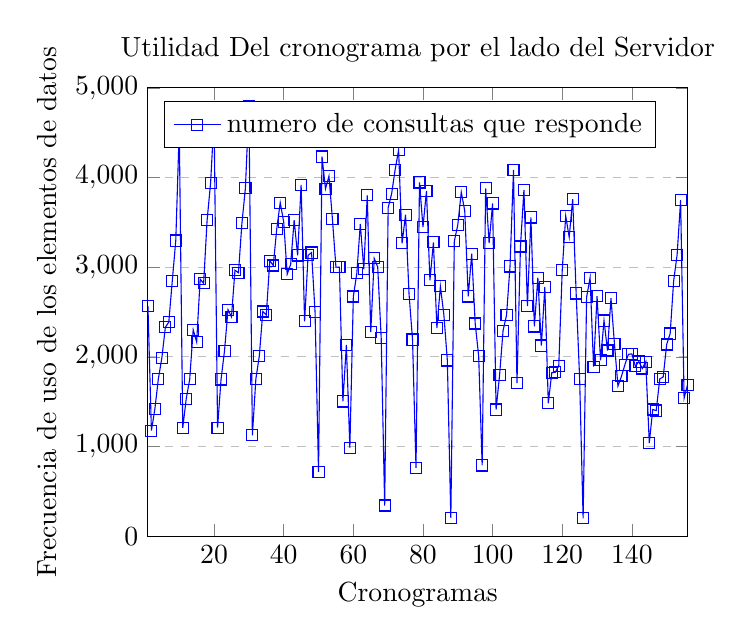
\begin{tikzpicture}
\begin{axis}[
    title={Utilidad Del cronograma por el lado del Servidor},
    xlabel={Cronogramas},
    ylabel={Frecuencia de uso de los elementos de datos},
    xmin=1, xmax=156,
    ymin=0, ymax=5000,
    xtick={},
    ytick={},
    legend pos=north west,
    ymajorgrids=true,
    grid style=dashed,
]

\addplot[
    color=blue,
    mark=square,
    ]
    coordinates {
%UTILIDAD TOTAL
%(cronograma, numero cues que usan al cronograma)
(1,2569)
(2,1177)
(3,1420)
(4,1757)
(5,1988)
(6,2329)
(7,2388)
(8,2850)
(9,3297)
(10,4538)
(11,1207)
(12,1532)
(13,1750)
(14,2302)
(15,2166)
(16,2867)
(17,2820)
(18,3525)
(19,3938)
(20,4671)
(21,1210)
(22,1748)
(23,2068)
(24,2527)
(25,2446)
(26,2966)
(27,2938)
(28,3491)
(29,3882)
(30,4801)
(31,1124)
(32,1753)
(33,2012)
(34,2506)
(35,2468)
(36,3072)
(37,3019)
(38,3427)
(39,3720)
(40,3504)
(41,2922)
(42,3032)
(43,3524)
(44,3131)
(45,3919)
(46,2396)
(47,3132)
(48,3163)
(49,2503)
(50,718)
(51,4234)
(52,3875)
(53,4016)
(54,3533)
(55,3001)
(56,2999)
(57,1503)
(58,2132)
(59,984)
(60,2673)
(61,2933)
(62,3482)
(63,2978)
(64,3802)
(65,2275)
(66,3098)
(67,3003)
(68,2211)
(69,342)
(70,3663)
(71,3820)
(72,4086)
(73,4306)
(74,3267)
(75,3586)
(76,2700)
(77,2193)
(78,761)
(79,3945)
(80,3447)
(81,3850)
(82,2854)
(83,3277)
(84,2322)
(85,2786)
(86,2470)
(87,1960)
(88,203)
(89,3288)
(90,3472)
(91,3837)
(92,3628)
(93,2674)
(94,3151)
(95,2372)
(96,2008)
(97,789)
(98,3879)
(99,3269)
(100,3711)
(101,1412)
(102,1794)
(103,2291)
(104,2464)
(105,3008)
(106,4084)
(107,1707)
(108,3231)
(109,3862)
(110,2566)
(111,3555)
(112,2339)
(113,2884)
(114,2126)
(115,2779)
(116,1483)
(117,1824)
(118,1828)
(119,1899)
(120,2966)
(121,3570)
(122,3335)
(123,3759)
(124,2707)
(125,1755)
(126,199)
(127,2666)
(128,2884)
(129,1891)
(130,2677)
(131,1961)
(132,2405)
(133,2071)
(134,2654)
(135,2145)
(136,1675)
(137,1782)
(138,1912)
(139,2028)
(140,2033)
(141,1894)
(142,1948)
(143,1871)
(144,1945)
(145,1039)
(146,1413)
(147,1401)
(148,1753)
(149,1776)
(150,2138)
(151,2260)
(152,2846)
(153,3139)
(154,3747)
(155,1539)
(156,1690)
    };
    \legend{numero de consultas que responde}

\end{axis}
\end{tikzpicture}

